\section{The Distribution Of Prefix Lengths}

So far we haven't worried much about the length of the prefixes we're producing. None of the computations we've performed gave any reason for particular concern since anytime there was a potentially unbounded iteration going on, the number of iterations was roughly geometrically distributed. We'll now double check this intuition.

Let's start with some numerical evidence. We have already seen how to compute the probabilities of specific prefixes. This allows us to estimate the expected length of prefixes of the examples we've seen so far. The following results take into account all unpadded prefixes of length 15 or less:
\begin{itemize}
	\item Standard normal distribution $\approx 0.1846$
	\item Exponential distribution ($\lambda = 1$) $\approx 0.5626$
	\item Sinusoidal distribution $\approx 3.4979$
\end{itemize}
This isn't a bad start. But computing these values is fairly inconvenient if one doesn't already have the required program at hand. A more general approach seems desirable. To see what kind of general result is possible it's best to first consider what sort of distribution might cause the corresponding prefix lengths to run away and become arbitrarily long.

Consider the continuous distribution whose support is only on the interval $[0,2^{-n}]$. Sampling a prefix from that interval will necessitate producing at least $n$ digits, since all shorter prefixes run the risk of producing a number outside the target interval when concatenating random bits to it. Hence the expected prefix length can in principle become arbitrarily long.

Note however, that in order for such a density to still integrate to 1 it will have to be spiked extremely sharply. This suggests that we might be able to make progress by adding an assumption that prevents such sharp spikes. One natural way of doing this is by assuming that the derivative of the density be bounded in absolute value or, slightly more generally, that the density be globally Lipschitz-continuous.

\begin{definition}{(Lipschitz-Continuity)}
	We say that a function $f:\mathbb{R}\rightarrow\mathbb{R}$ is (globally) Lipschitz-continuous if there exists a $K$ such that for all $x, y$
	\[
	|f(x)-f(y)| \leq K|x-y|\,. \qquad K,x,y\in\mathbb{R}
	\]
	We'll also say that such a function is $K$-Lipschitz. And we'll often say that a function is $K$-Lipschitz only on some finite interval $[a,b]$.
\end{definition}

But even after having added the assumption that the density be Lipschitz-continuous, there's still another issue lurking. The problem is that, instead of being sharply spiked on the interval $[0,2^{-n}]$, the density might also manage to integrate to 1 by repeating many little spikes on the intervals $[k, k+2^{-n}]$ for $k \in \mathbb{Z}$. How do we also rule out these?

Again, the most natural way of preventing such pathologies is by insisting that the density have support only on some restricted interval $[a,b]$. However, in contrast with the assumption that $f$ be Lipschitz-continuous, which seemed fairly benign, this new assumption raises the question whether we're throwing out the baby with the bathwater. After all, many of our most cherished distributions, such as the normal or the exponential distribution, \textit{don't} have their densities restricted to an interval.

The way we'll address this issue is by splitting up the real line into intervals of unit length. We then condition on the prefix falling into one of these intervals, use the bounds we obtain for each interval, and put the whole thing back together. We'll see an example of this at the end of this section. But for now, we'll continue by establishing the following.

\begin{proposition}\label{a}
	Let $f$ be a probability density and let $R$ be a unpadded prefix for $f$. Assuming that $f$ is $K$-Lipschitz and has support $[i,i+1]$ where $i\in\mathbb{Z}$ it follows that  
	\[
	\pr{}{\#R \leq n} >1-2^{-n}K
	\]
\end{proposition}
\begin{proof}
First, without loss of generality we'll assume that $i=0$. Now consider figures \ref{fig:normal_bin_cover_2} and \ref{fig:normal_bin_cover_riemann}. As these two figures demonstrate, the area covered by the probabilities of length $n$ or less prefixes is identical to the area covered by the lower Riemann sum corresponding to the partition
\[
\{k\cdot2^{-n}|k\in\mathbb{Z}\}\,.
\]

\begin{figure}[h]
	\centering
	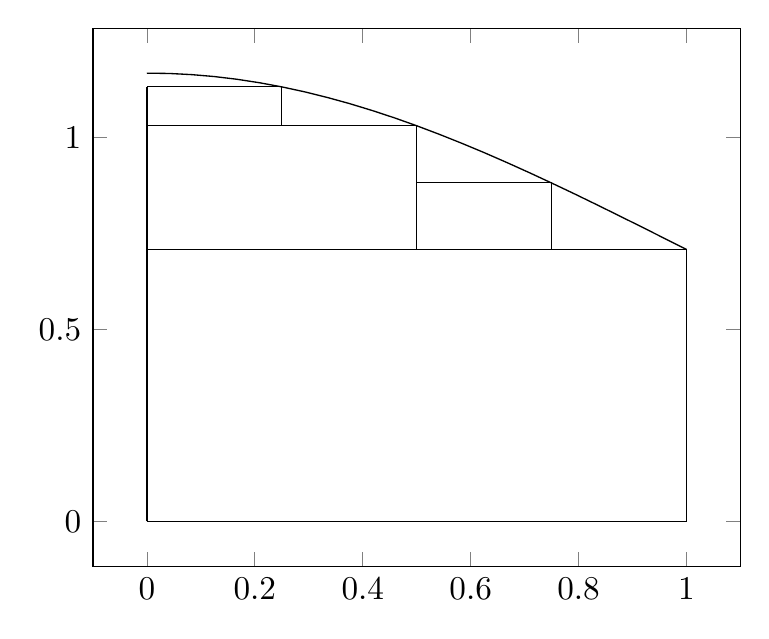
\begin{tikzpicture}[scale=1.2]
\begin{axis}
\addplot[draw=none] coordinates {(0,0)};
\addplot[domain=0:1] {e^(-x^2/2)/0.85624};
\draw (axis cs: 0, 0) -- (axis cs: 1, 0);
\draw (axis cs: 0, 0) -- (axis cs: 0, 0.7088752307384394);
\draw (axis cs: 1, 0) -- (axis cs: 1, 0.7088752307384394);
\draw (axis cs: 0, 0.7088752307384394) -- (axis cs: 1, 0.7088752307384394);
\draw (axis cs: 0, 0.7088752307384394) -- (axis cs: 0, 1.0314073738483691);
\draw (axis cs: 1/2, 0.7088752307384394) -- (axis cs: 1/2, 1.0314073738483691);
\draw (axis cs: 0, 1.0314073738483691) -- (axis cs: 1/2, 1.0314073738483691);
\draw (axis cs: 1/2, 0.7088752307384394) -- (axis cs: 1/2, 0.7088752311585824);
\draw (axis cs: 1, 0.7088752307384394) -- (axis cs: 1, 0.7088752311585824);
\draw (axis cs: 1/2, 0.7088752311585824) -- (axis cs: 1, 0.7088752311585824);
\draw (axis cs: 0, 1.0314073738483691) -- (axis cs: 0, 1.132779392052711);
\draw (axis cs: 1/4, 1.0314073738483691) -- (axis cs: 1/4, 1.132779392052711);
\draw (axis cs: 0, 1.132779392052711) -- (axis cs: 1/4, 1.132779392052711);
\draw (axis cs: 1/4, 1.0314073738483691) -- (axis cs: 1/4, 1.0314073740037737);
\draw (axis cs: 1/2, 1.0314073738483691) -- (axis cs: 1/2, 1.0314073740037737);
\draw (axis cs: 1/4, 1.0314073740037737) -- (axis cs: 1/2, 1.0314073740037737);
\draw (axis cs: 1/2, 0.7088752311585824) -- (axis cs: 1/2, 0.8822094784609293);
\draw (axis cs: 3/4, 0.7088752311585824) -- (axis cs: 3/4, 0.8822094784609293);
\draw (axis cs: 1/2, 0.8822094784609293) -- (axis cs: 3/4, 0.8822094784609293);
\draw (axis cs: 3/4, 0.7088752311585824) -- (axis cs: 3/4, 0.7088752308298532);
\draw (axis cs: 1, 0.7088752311585824) -- (axis cs: 1, 0.7088752308298532);
\draw (axis cs: 3/4, 0.7088752308298532) -- (axis cs: 1, 0.7088752308298532);
\end{axis}
\end{tikzpicture}
	\caption{The normal distribution on the interval $[0,1]$ divided up according to which sections produce distinct prefixes (prefixes up to length 2 have been plotted)}
	\label{fig:normal_bin_cover_2}\vspace{2em}
	
	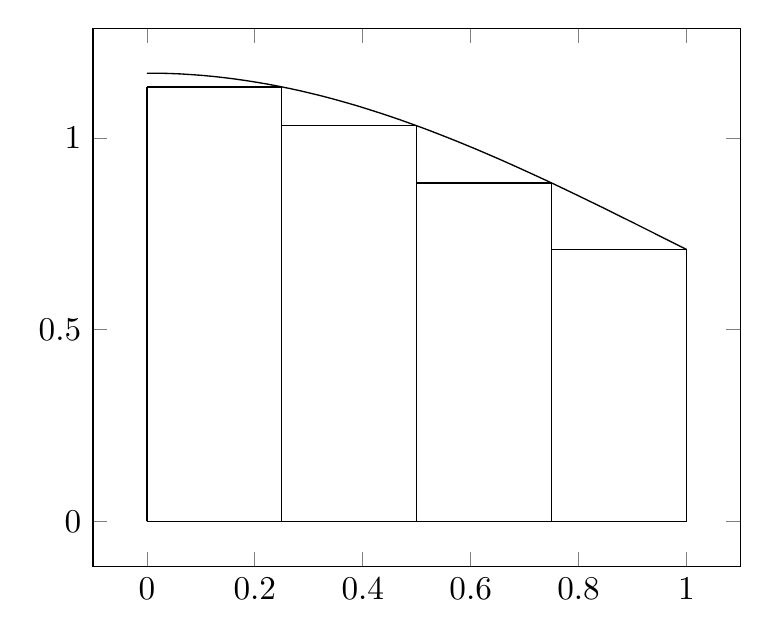
\begin{tikzpicture}[scale=1.2]
\begin{axis}
\addplot[draw=none] coordinates {(0,0)};
\addplot[domain=0:1,samples=50] {e^(-x^2/2)/0.855624};
\draw (axis cs: 0, 0) -- (axis cs: 1, 0);
\draw (axis cs: 0, 0) -- (axis cs: 0, 0.7088752307384394);
\draw (axis cs: 1, 0) -- (axis cs: 1, 0.7088752307384394);
\draw (axis cs: 0, 0) -- (axis cs: 0, 1.0314073738483691);
\draw (axis cs: 1/2, 0) -- (axis cs: 1/2, 1.0314073738483691);
\draw (axis cs: 1/2, 0) -- (axis cs: 1/2, 0.7088752311585824);
\draw (axis cs: 1, 0) -- (axis cs: 1, 0.7088752311585824);
\draw (axis cs: 0, 0) -- (axis cs: 0, 1.132779392052711);
\draw (axis cs: 1/4, 0) -- (axis cs: 1/4, 1.132779392052711);
\draw (axis cs: 0, 1.132779392052711) -- (axis cs: 1/4, 1.132779392052711);
\draw (axis cs: 1/4, 0) -- (axis cs: 1/4, 1.0314073740037737);
\draw (axis cs: 1/2, 0) -- (axis cs: 1/2, 1.0314073740037737);
\draw (axis cs: 1/4, 1.0314073740037737) -- (axis cs: 1/2, 1.0314073740037737);
\draw (axis cs: 1/2, 0) -- (axis cs: 1/2, 0.8822094784609293);
\draw (axis cs: 3/4, 0) -- (axis cs: 3/4, 0.8822094784609293);
\draw (axis cs: 1/2, 0.8822094784609293) -- (axis cs: 3/4, 0.8822094784609293);
\draw (axis cs: 3/4, 0) -- (axis cs: 3/4, 0.7088752308298532);
\draw (axis cs: 1, 0) -- (axis cs: 1, 0.7088752308298532);
\draw (axis cs: 3/4, 0.7088752308298532) -- (axis cs: 1, 0.7088752308298532);
\end{axis}
\end{tikzpicture}
	\caption{This figure is identical to figure 26 except that the thinnest rectangles have been vertically extended}
	\label{fig:normal_bin_cover_riemann}
\end{figure}

So we can estimate the probability that a prefix has length $n$ or less by simply estimating this lower Riemann sum. In particular, we'll do so by finding an upper bound for $\pr{}{\#P>n}$, which is equivalent to the error of the lower Riemann sum.

Let $L_n$ be the lower Riemann sum with the aforementioned partition. And let $m_k$ and $M_k$ be the min and max respectively of $f$ on the interval $[k2^{-n}, (k+1)2^{-n}]$. Then $L_n$ consists of terms that are each of the form
\[
\underbrace{2^{-n}}_{\text{width}} \cdot \underbrace{m_k}_{\text{height}}\,.
\]
On the other hand, the actual area under the curve on such an interval is at most
\[
2^{-n} \cdot M_k\,.
\]
Thus the error on each interval is at most $2^{-n}(M_k-m_k)$. Using the fact that $f$ is $K$-Lipschitz we then get
\[
2^{-n}(M_k-m_k)\leq 2^{-2n}K
\]
as an upper bound on each interval. Thus, the total error is bounded as follows:
\[
\int_0^1f(x)\,dx - L_n \leq 2^n\cdot 2^{-2n}K = 2^{-n}K\,.
\]
In other words $\pr{}{\#R>n}\leq2^{-n}K$. Hence $\pr{}{\#R\leq n}>1-2^{-n}K$.
\end{proof}

Also note that all our inequalities become equalities in the case where $f$ is a straight line. The bound on expected values is now essentially just a corollary.

\begin{proposition}
	Using the previous definitions and assumptions we have for the expected unpadded prefix length 
	\[
	\ev{}{\#R} \leq K
	\]
\end{proposition}
\begin{proof}
The proof is straightforward:
\[
\begin{split}
	\ev{}{\#R} & =\sum_{n=0}^\infty n\,\pr{}{\#R=n}\\
			 & =\sum_{n=1}^\infty n\left(\pr{}{\#R\geq n} - \pr{}{\#R\geq n+1}\right)\\
			 & =\sum_{n=1}^\infty \pr{}{\#R\geq n}\\
			 & \leq\sum_{n=1}^\infty 2^{-n}K\\
			 & = K\,.
\end{split}
\]
\end{proof}

Finally, we can apply this to a distribution with unbounded support.

\begin{proposition}
	Using the previous definitions and assumptions, but where $f$ has arbitrary support we have
	\[
	\ev{}{\#R}\leq\sum_{i\in\mathbb{Z}} K_i
	\]
	where $K_i$ is the Lipschitz constant of $f$ corresponding to the interval $[i,i+1]$.
\end{proposition}
\begin{proof}
We'll use the fact that the Lipschitz constant for $f$ conditioned on the interval $[i,i+1]$ is the same as the Lipschitz constant of $f$ itself on that interval, but normalized by dividing it by $\pr{}{R\in[i,i+1]})$.

\[
\begin{split}
	\ev{}{\#R} & =\sum_{i\in\mathbb{Z}} \ev{}{\#R|R\in[i,i+1]}\cdot\pr{}{R\in[i,i+1]})\\
			   & \leq\sum_{i\in\mathbb{Z}} \frac{K_i}{\pr{}{R\in[i,i+1]})}\cdot\pr{}{R\in[i,i+1]})\\
			   & = \sum_{i\in\mathbb{Z}} K_i
\end{split}
\]
\end{proof}

The infinite sum $\sum_{i\in\mathbb{Z}} K_i$ may look intimidating. But in all but the most pathological cases this will be a quite manageable finite value. For example, we can bound the sum using the absolute values of the first and second derivatives of $f$.

\begin{lemma}
	Given a differentiable function $f : \mathbb{R} \rightarrow \mathbb{R}$ we have
	\[
	\sup_{x\in[a,b]}|f(x)|\leq\int_a^b\frac{|f(x)|}{b-a}+|f'(x)|\,dx
	\]
	 for any $a\leq b$ where $a,b\in\mathbb{R}$.
\end{lemma}
\begin{proof}
Because $f$ is differentiable, it is also continuous. So there exists an $x_1$ such that
\[
f(x_1)=\sup_{x\in[a,b]}|f(x)|\,. 
\]
Furthermore, by the mean value theorem, there exists an $x_2\in[a,b]$ such that
\[
f(x_2)=\frac{1}{b-a}\int_a^b f(x)\,dx\,.
\]
Therefore
\[
\begin{split}
\sup_{x\in[a,b]}|f(x)|-\left|\frac{1}{b-a}\int_a^b f(x)\,dx\right|
& = |f(x_1)|-|f(x_2)|\\
& \leq |f(x_1)-f(x_2)|\\
& = \left|\int_{x_2}^{x_1}f'(x)\,dx\right|\\
& \leq \int_{x_2}^{x_1}|f'(x)|\,dx\\
& \leq \int_{a}^{b}|f'(x)|\,dx\\
\end{split}
\]
which yields
\[
\sup_{x\in[a,b]}|f(x)| \leq \left|\frac{1}{b-a}\int_a^b f(x)\,dx\right|+\int_{a}^{b}|f'(x)|\,dx\leq\int_a^b\frac{|f(x)|}{b-a}+|f'(x)|\,dx\,.
\]
\end{proof}

This lemma is immediately applicable to expected prefix lengths.

\begin{proposition}
	Using the previous definitions and assumptions, if $f$ is twice differentiable, we have
	\[
	\ev{}{\#R}\leq\sum_{i\in\mathbb{Z}} K_i\leq \int_\mathbb{R}|f'(x)|+|f''(x)|\,dx
	\]
\end{proposition}
\begin{proof}
For a differentiable function $f$ the Lipschitz constant $K_i$ is nothing but $\sup_{x\in[i,i+1]}|f'(x)|$. So we can simply apply the previously established bound to each $K_i$ and sum the results.
\end{proof}

Because $f$ integrates to 1, the only way this upper bound could fail to be finite is if $f$ oscillates with exceedingly vanishing amplitude -- aberrant to say the least.

Let's conclude this section by taking the standard normal distribution as an example. First, the sum of the $K_i$: Because the normal distribution is symmetric we can just sum over the positive intervals and double the result. For the first interval $[0,1]$ the maximum slope in absolute value is attained at the right-hand side. For all further intervals it is attained at the left-hand side. Therefore the expected prefix length is bounded by
\[
2\left(|\varphi'(1)|+\sum_{i=1}^\infty |\varphi'(i)|\right) \approx 1.2115\,.
\]
Using the integrals as an upper bound instead produces
\[
\sqrt{\frac{2}{\pi}}+2\,\sqrt{\frac{2}{e\cdot\pi}}\approx 1.7658\,.
\]

Similar considerations for both the exponential and the sinusoidal distribution allow us to give the following summary.
\begin{center}
\begin{tabular}{l | c | c | c}
& numerical estimate & $\sum_i K_i$ & $\int |f'| + |f''|\,dx$\\
\hline
standard normal & 0.1846 & 1.2115 & 1.7658\\
exponential & 0.5626 & 1.5820 & 2\\
sinusoidal & 3.4979 & 12.5664 & 108.5310\\
\end{tabular}
\end{center}
These examples showcase both scenarios where the upper bounds are reasonably tight and where they are not.



